\section{Introduction}\label{sec:introduction}
\subsection{Vue d'ensemble}

Un système d'exploitation est constitué d'un noyau auquel vient s'ajouter le code d'une distribution.
Le développeur d'un système d'exploitation doit abstraire le fonctionnement des périphériques afin d'offre un interface de programmation au programmeur.
La gestion des ressources et les communications avec les différents périphériques est gérée par le système d'exploitation.

\subsection{Abstractions de programmation}

Un système d’exploitation peut être perçu comme exposant une interface de programmation système aux programmes qui tournent sur une machine.

\begin{figure}[h!]
    \centering
    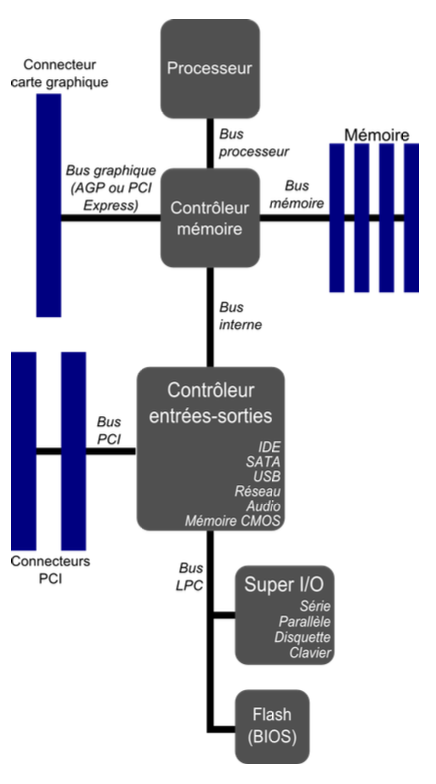
\includegraphics[width=0.2\textwidth]{Images/View/view.png}
    \caption{View}
    \label{fig:myimage}
  \end{figure}
  

\subsection{Processeur}


Le \textbf{processeur} exécute les instructions et réalise les traitements. Il est caractérisé par son jeu d'instructions (Instruction Set Architecture), qui définit les instructions exécutables et leur format d'encodage (opcode et opérandes). Les instructions sont classées en plusieurs types :
\begin{itemize}
    \item Arithmétique (e.g. \texttt{add}, \texttt{div})
    \item Logique (e.g. \texttt{and})
    \item Accès mémoire (e.g. \texttt{lw}, \texttt{sw})
    \item Instructions système
\end{itemize}

Les processeurs modernes utilisent une structure de pipeline, permettant à différentes instructions d'occuper simultanément différentes parties du pipeline. Deux types principaux d'architecture de jeu d'instructions existent :
\begin{itemize}
    \item RISC (Reduced Instruction Set Computer)
    \item CISC (Complex Instruction Set Computer)
\end{itemize}

Les responsabilités de gestion du processeur en collaboration avec le système d'exploitation incluent :
\begin{itemize}
    \item Surveillance de l'exécution des instructions
    \item Répartition du temps processeur entre différents programmes
\end{itemize}


\subsubsection{Exécution de programme}

La première responsabilité de gestion consiste à surveiller l'exécution des instructions d'un programme utilisant le processeur. Le système d'exploitation et les programmes se partagent le processeur, nécessitant la suspension de l'exécution en cours lors d'un évènement particulier. Le processeur peut réagir de différentes manières :

\begin{itemize}
    \item \textbf{Mauvais comportement} : déroutement vers une fonction du système d'exploitation pour traiter des erreurs telles qu'une division par zéro, un accès mémoire invalide ou une tentative d'exécuter une instruction privilégiée.
    \item \textbf{Anomalie non fatale} : correction des circonstances ayant provoqué l'anomalie et reprise de l'exécution.
    \item \textbf{Appel système} : branchement vers une fonction du système d'exploitation pour des demandes comme l'obtention de mémoire ou l'écriture dans un fichier.
    \item \textbf{Interruption externe} : traitement d'une interruption provenant d'un périphérique externe. Par exemple, une interruption du clavier nécessite de communiquer avec le contrôleur du clavier pour identifier la touche concernée et le programme destinataire.
\end{itemize}


\subsubsection{Ordonnancement de programmes}

La seconde responsabilité du système d'exploitation est de répartir le temps processeur entre les programmes. L'ordonnancement sélectionne le prochain programme à exécuter lorsque le processeur est libre. Différentes stratégies sont utilisées selon le type de système et la charge de travail. Les métriques d'évaluation incluent la minimisation du temps d'exécution moyen et l'adéquation entre les besoins du programme et le temps processeur alloué.


\subsection{Mémoire}

La mémoire stocke les données de travail des programmes et est organisée en une hiérarchie :
\begin{itemize}
    \item \textbf{Caches} (e.g. L1, L2) : Intermédiaires entre les registres et la mémoire principale, stockant temporairement les données fréquemment accédées (principe de localité).
    \item \textbf{Mémoire principale} (e.g. RAM, GPU) : Stocke les données de travail (e.g. tableaux, variables, stack) lorsqu'il n'y a pas de registres disponibles.
    \item \textbf{Mémoire secondaire} (e.g. HDD, SSD) : Utilisée comme espace temporaire (swap) lorsque la mémoire principale est pleine.
\end{itemize}

L'allocation dynamique permet de gérer la mémoire de manière flexible. La mémoire virtuelle charge/décharge les données non actives pour pallier les limitations de la mémoire physique (e.g. adressage 32 bits, 0x00000000 à 0xffffffff).


\subsubsection{Protection de la mémoire}

Le système d'exploitation contrôle les accès mémoire pour garantir qu'un programme n'accède qu'à sa propre mémoire, évitant ainsi la lecture ou la modification de données sensibles (e.g. clefs de chiffrement). Le processeur vérifie les accès mémoire selon les descriptions des espaces mémoire accessibles à chaque programme, mises à jour par le système d'exploitation.

\begin{itemize}
    \item \textbf{Adresse valide} : Accessible au programme, l'accès est accordé (e.g. \texttt{lw}, \texttt{sw}).
    \item \textbf{Adresse indisponible} : Accessible mais non présente en mémoire principale, nécessite un chargement depuis la mémoire secondaire.
    \item \textbf{Adresse invalide} : Hors de l'espace accessible, entraîne l'arrêt du programme.
\end{itemize}



\subsubsection{Répartition de la mémoire}

La seconde responsabilité de gestion est la répartition de la mémoire principale entre les différents programmes. Cela inclut la représentation et le suivi des portions de mémoire (libres ou non) et l'identification d'une portion adéquate pour satisfaire une demande d'allocation dynamique.

\subsection{Stockage}

Le stockage préserve les données produites par un programme au-delà de son exécution. Une fois le programme terminé, sa mémoire est libérée et peut être allouée à un autre programme. La notion de fichier assure la pérennité des données, malgré la diversité des supports physiques adaptés à différents scénarios d’utilisation :

\begin{itemize}
    \item \textbf{HDD} : Disque dur, bon marché, accès lent, organisé en plateaux, cylindres, têtes, et secteurs.
    \item \textbf{SSD} : Disque à état solide, rapide, coût plus élevé, organisé en blocs et pages.
    \item \textbf{Bande magnétique} : Grande capacité, fiable, utilisé pour les backups.
\end{itemize}

Un système de fichiers met en place une abstraction pour accéder au stockage, en représentant les fichiers et répertoires et leurs méta-données (e.g. taille, dates, permissions). Il garantit également la cohérence des écritures et réduit la possibilité de corruption des données.

\subsection{Typologie des systèmes}

Les types de systèmes influencent la conception des systèmes d'exploitation :

\begin{itemize}
    \item \textbf{Mainframe} : Exécute des jobs réguliers avec des E/S intensives (e.g. calcul des fiches de paie). Supporte un grand volume de transferts et offre une gestion de timesharing pour plusieurs utilisateurs.
    \item \textbf{Serveur} : Fournit des services aux utilisateurs distants (e.g. serveur d'impression), gère les ressources et la facturation.
    \item \textbf{Personal Computer} : Interaction humaine via interface graphique, exécution simultanée de plusieurs programmes, interactivité centrale (mesurée par la latence entre l'action et la réaction).
    \item \textbf{Système mobile} (e.g. tablette, smartphone) : Contraintes de ressources, économie d'énergie cruciale, processeur et mémoire limités, alimentation par batterie.
    \item \textbf{Système embarqué} (e.g. TV, voiture) : Logiciel prédéterminé pour une machine spécifique, pas de flexibilité pour l'installation d'applications supplémentaires.
    \item \textbf{Système de senseurs} : Surveille des paramètres environnementaux (e.g. température, humidité), transmet les données à un central, optimisé pour faible consommation d'énergie.
    \item \textbf{Système temps-réel} : Respect des échéances crucial, priorisation des tâches, gestion précise du temps pour aligner les traitements avec l'environnement.
\end{itemize}


\subsection{Architecture}

Un système d'exploitation inclut le code, les données, et la stack, similaires à un programme classique. Il utilise des instructions système nécessitant des niveaux de privilège spécifiques, et le noyau gère les ressources.

\begin{itemize}
    \item \textbf{Noyau monolithique} : Code dans un fichier unique, exécuté au plus haut niveau de privilège. Exemple : système avec configuration matérielle fixe.
    \item \textbf{Noyau modulaire} : Base toujours en mémoire, modules chargés/déchargés selon les besoins. Exemple : Linux.
    \item \textbf{Microkernel} : Composantes exécutées à des niveaux de privilège réduits pour éviter les compromissions. Un serveur de ré-incarnation gère les erreurs fatales. Exemple : MINIX3.
    \item \textbf{Exokernel} : Gestion des ressources laissée aux programmes, le noyau assure uniquement la protection et l'isolation. Exemple : machines virtuelles.
\end{itemize}

